\chapter{Mạng Nơ-ron Tích chập (Convolutional Neural Network)}

\section{Giới thiệu mạng nơ-ron tích chập}
\subsection{Lịch sử mạng nơ-ron tích chập}

\hspace{\parindent} \textit{\textbf{Mạng Nơ-ron tích chập}} (Convolutional Neural Network, còn được viết tắt là CNN hay ConvNet) là một trong những nền tảng quan trọng của chuyên ngành \textit{Thị giác máy tính} (Computer Vision) nói riêng, hay của ngành \textit{Học sâu} (Deep learrning) nói chung. CNN được chuyên dùng cho các bài toán liên quan đến hình ảnh như phân loại, phân tích hình ảnh (image classification) hay nhận diện khuôn mặt (facial recognition).

Những ý tưởng sơ khai đầu tiên để hình thành nên một mạng nơ-ron tích chập như hiện nay đã bắt nguồn từ những năm 50 và 60 của thế kỷ trước. Trong một bài báo khoa học của 2 nhà nghiên cứu David H. Hubel và Torsten Wiesel về những vùng cảm thụ của vỏ não thị giác (receptive fields of visual cortex), tác giả đã nêu ra cách xử lý hình ảnh của các tế bào thị giác chính là nhận biết các \textit{cạnh thẳng} (straight edges). Các tế bào thị giác được chia làm 2 loại, đó là \textit{tế bào tối giản} (simple cell) và \textit{tế bào phức hợp} (complex cell). 2 nhà khoa học cũng đưa ra mô hình xếp tầng (cascading model) để lý giải cách nhận dạng mẫu (pattern recognition) của 2 loại tế bào này [\ref{refer:15}].

Đến năm 1979, nhà khoa học dữ liệu người Nhật Bản Kunihiko Fukushima đưa ra khái niệm "Neocognitron", đây được xem là mạng Nơ-ron tích chập nguyên thủy của ngành Thị giác máy tính. Dựa trên những ý tưởng của Hubel và Wiesel, các \textit{tầng} (layer) của Neocognitron được chia làm 2 loại cơ bản: tầng S-cells được sử dụng để trích xuất các \textit{thuộc tính cục bộ} (local feature) của hình ảnh, tương đương với simple cell (dùng để xử lý các đường thẳng cơ bản); trong khi C-cells được dùng để giảm thiểu các sai sót khi kết hợp nhiều thuộc tính cục bộ với nhau (tương đương với complex cell). Các \textit{thuộc tính cục bộ }được tích hợp dần và phân loại ở các tầng sâu hơn. Từ đó máy tính sẽ nhận dạng được các đặc điểm khác nhau của hình ảnh trong quá trình học và có thể phân loại được hình ảnh dựa trên các \textit{bộ lọc} khác nhau (filter). Đến nay thì những ý tưởng cơ bản của các mạng CNN hiện đại vẫn dựa trên mạng Neocognitron này [\ref{refer:16}].

Có thể thấy, những ý tưởng khởi phát của CNN đã có từ cách đây khá lâu (gần 30 năm), nhưng sự trỗi dậy của ngành Học sâu, cụ thể hơn là Thị giác máy tính chỉ thực sự bắt đầu từ những năm đầu của Thế kỷ XXI với sự phát triển của ngành công nghiệp Trò chơi điện tử. Các card đồ họa ngày càng được nâng cấp để nâng cao trải nghiệm chơi game cho người dùng, mà cốt lõi chính là việc tăng cường khả năng tính toán của các bộ xử lý đồ họa (GPU- Graphic Processing Units). Thoạt nghe thì có vẻ CNN không dính dáng tới GPU lắm vì chúng thuộc 2 chuyên ngành khác biệt, nhưng thực tế chúng đều hoạt động dựa trên các thao tác với ma trận (matrix manipulation). Hình ảnh là một ma trận các điểm ảnh (pixel), còn video thì ghép nối nhiều hình ảnh khác nhau trong một khoảng thời gian nhất định (60 frame per second chẳng hạn) để tạo nên những chuyển động. Do tính chất này, GPU được cải thiện sao cho việc tính toán các ma trận pixel được diễn ra nhanh nhất có thể, điều này vô tình khiến các mạng nơ-ron nhân tạo được hưởng lợi rất nhiều.

\subsection{Đặc tính cơ bản của mạng nơ-ron tích chập}

\hspace{\parindent} Vậy tại sao mạng nơ-ron tích chập lại được sử dụng phổ biến cho các bài toán phân tích hình ảnh? Câu trả lời đến từ một bản chất tự nhiên của CNN, đó là khả năng \textit{rút trích thuộc tính ẩn} (latent feature extraction) cực kỳ tốt. Để có thể nhận biết rõ hơn về tầm quan trọng của việc rút trích được những thuộc tính ẩn,ta hãy cùng phân tích ví dụ dưới đây về mối liên hệ giữa cách thức con người suy nghĩ để đưa ra quyết định và quá trình học của mạng nơ-ron nhân tạo.

\begin{figure}[!h]
	\centering
		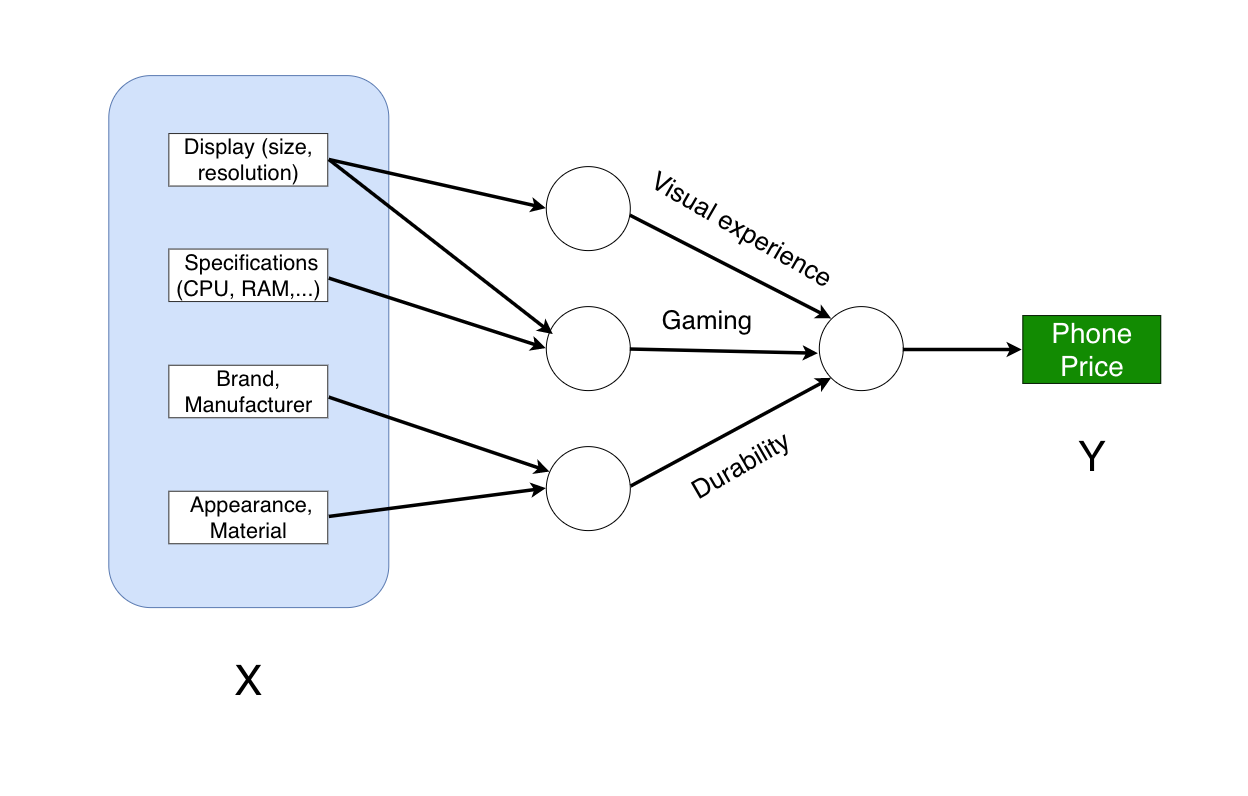
\includegraphics[width=1.0\columnwidth]{books/artificial-neural-network/chapter05/figure/CNN_human_thinking.png}
		\centering
	\caption{Hình ảnh minh họa phân tích của nhà phân phối điện thoại thông minh}
	\label{fig:CNNHumanThinking}
\end{figure}

Hình \ref{fig:CNNHumanThinking} là một minh họa về quá trình phân tích và rút trích các thuộc tính ẩn để từ đó đưa ra quyết định định giá sản phẩm của một nhà phân phối điện thoại thông minh. Có thể thấy được giá trị đầu vào chính là những thông số thường được đi kèm với mỗi dòng điện thoại như màn hình, vi xử lý, RAM, hãng sản xuất,...Tuy nhiên, các thông số này không trực tiếp quyết định số tiền mà người dùng cần bỏ ra để sở hữu chiếc điện thoại. Bản thân người dùng khi mua một sản phẩm luôn có những yêu cầu nhất định và phù hợp cho cá nhân mình, chẳng hạn như độ bền, khả năng chiến game, trải nghiệm hiển thị,...

Như vậy, đối với nhà phân phối, họ cần rút trích được các thuộc tính tiềm ẩn của sản phẩm và có ý nghĩa đối với khách hàng của họ (cũng chính là nhu cầu người dùng) từ những thông số đầu vào tương đối vô nghĩa. Ví dụ như thông số màn hình (kích thước, độ phân giải, tấm nền) sẽ quyết định trải nghiệm thị giác; thông số màn hình cộng với thông số phần cứng như chip xử lý, bộ nhớ RAM sẽ quyết định trải nghiệm chơi game; hoặc hãng sản xuất, chất liệu và thiết kế của sản phẩm có thể ảnh hưởng đến độ bền. Từ đó, nhà phân phối đưa ra giá trị cho mỗi loại điện thoại sao cho phù hợp và bán chạy khi giới thiệu đến người dùng.


\begin{figure}[!h]
	\centering
		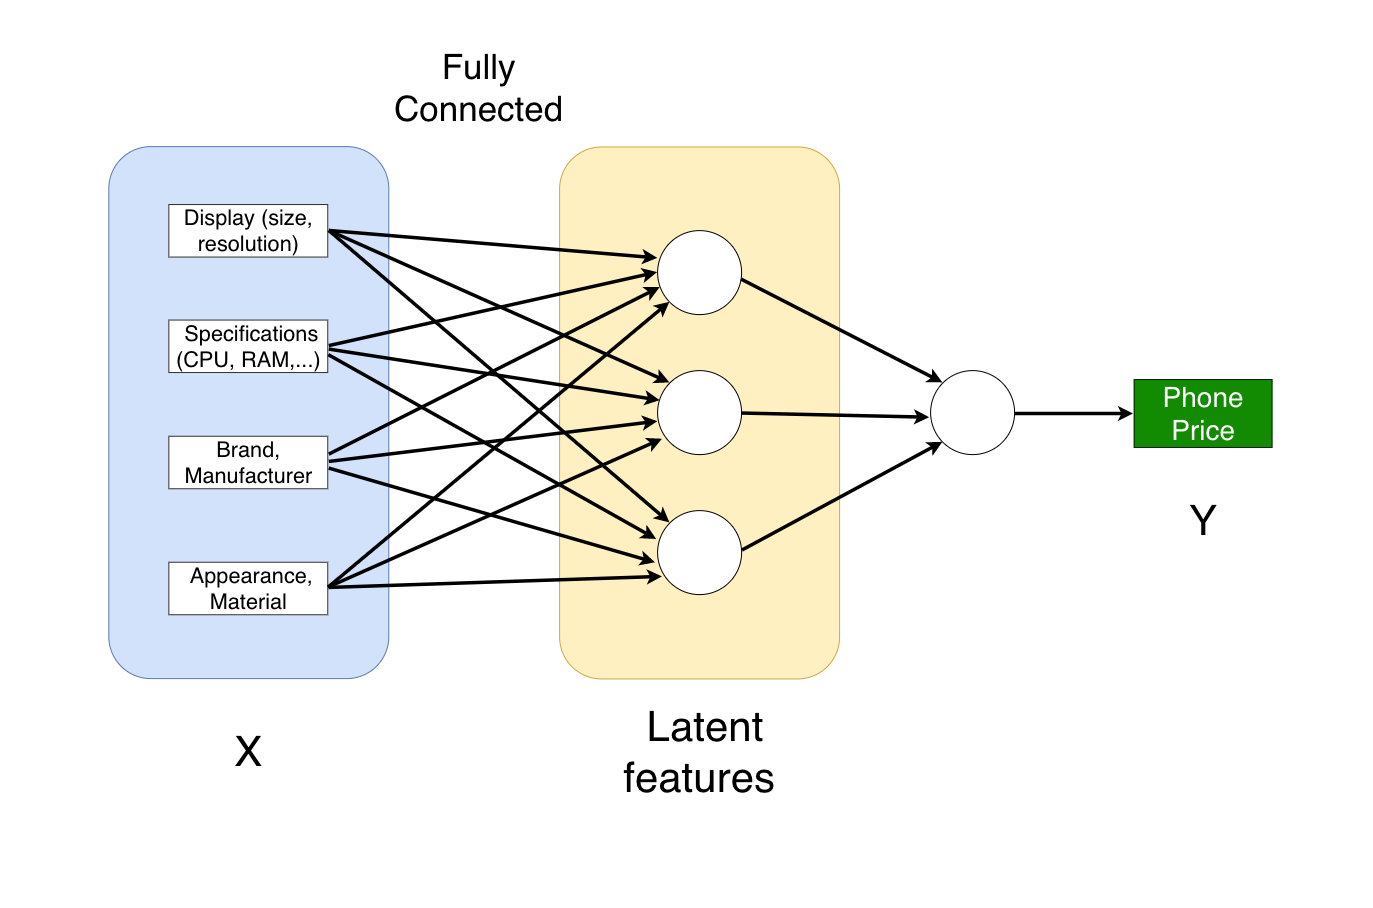
\includegraphics[width=1.0\columnwidth]{books/artificial-neural-network/chapter05/figure/CNN_machine_learning.png}
		\centering
	\caption{Hình ảnh minh họa quá trình học và trích xuất thuộc tính của một mạng nơ-ron}
	\label{fig:CNNMachineLearning}
\end{figure}

Hình \ref{fig:CNNMachineLearning} mô tả cơ bản quá trình học của một \textit{mạng nơ-ron nhân tạo} (neural network). Từ các giá trị đầu vào, mạng nơ-ron tiến hành các thao tác xử lý để trích xuất các \textit{thuộc tính tiềm ẩn} (latent features) của dữ liệu. Các thuộc tính này có thể tiếp tục được làm đầu vào cho các lớp sau đó cho đến khi tìm được kết quả cuối cùng.

Điểm đặc biệt của các thuộc tính tiềm ẩn được trích xuất từ mạng nơ-ron nhân tạo chính là thậm chí con người cũng đôi khi cũng không thể, hoặc rất khó khăn để suy luận ra được. Một ví dụ đơn giản chính là cách quá trình trẻ nhỏ nhận biết các con vật khác nhau. Dù thực tế chúng ta không được học về một định nghĩa hay lý thuyết cụ thể để phân biệt các loài vật, nhưng não bộ ta đã học được điều đó trong quá trình tiếp xúc trực tiếp hay gián tiếp. Do đó, khi được hỏi hãy liệt kê cụ thể các đặc điểm để phân biệt chó và mèo, đôi khi chúng ta cũng gặp không ít khó khăn để trích xuất các đặc điểm này, việc mà các mạng nơ-ron nhân tạo được thực hiện bởi máy tính lại thực hiện rất tốt.

Có nhiều mạng nơ-ron có thể đảm nhiệm tốt khả năng trích xuất thuộc tính. Tuy nhiên, đối với một số mạng nơ-ron sử dụng cơ chế \textit{kết nối đầy đủ} (fully-connected), có một vấn đề nảy sinh chính là số \textit{trọng số} (parameter) cần học là rất lớn bởi vì tất cả các giá trị đầu vào đều tham gia vào quá trình học của mỗi trọng số. Điều này có thể khiến cho máy học tương đối chậm. Với mạng nơ-ron tích chập, cơ chế \textit{chia sẻ trọng số} (shared weight) sẽ giúp tiết kiệm đáng kể chi phí với trọng số được học giảm rất nhiều. Chúng ta sẽ cùng phân tích về cơ chế chia sẻ trọng số này kỹ hơn ở phần sau của chương.

\section{Cách thức hoạt động của mạng nơ-ron tích chập}

\subsection{Phép tích chập (Convolution)}
\begin{figure}[!h]
	\centering
		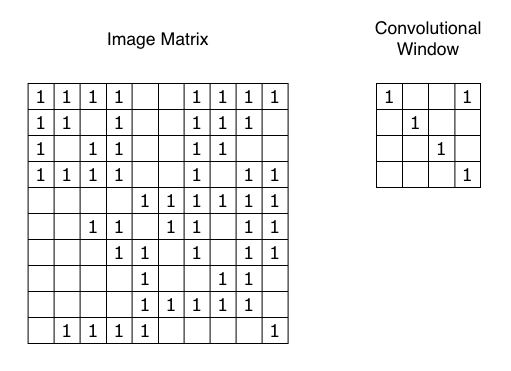
\includegraphics[width=0.8\columnwidth]{books/artificial-neural-network/chapter05/figure/convolution_example_sample.png}
		\centering
	\caption{Hình ảnh mô tả ma trận hình ảnh và cửa sổ tích chập}
	\label{fig:ConvolutionSample}
\end{figure}

\hspace{\parindent} Đúng như cái tên của CNN, phép tính \textit{tích chập} (convolution) chính là đặc trưng mạng nơ-ron này. Để có thể dễ dàng nắm bắt được ý tưởng của phép tích chập, ta hãy cùng phân tích ví dụ sau đây.

\begin{figure}[!h]
    	\centering
    		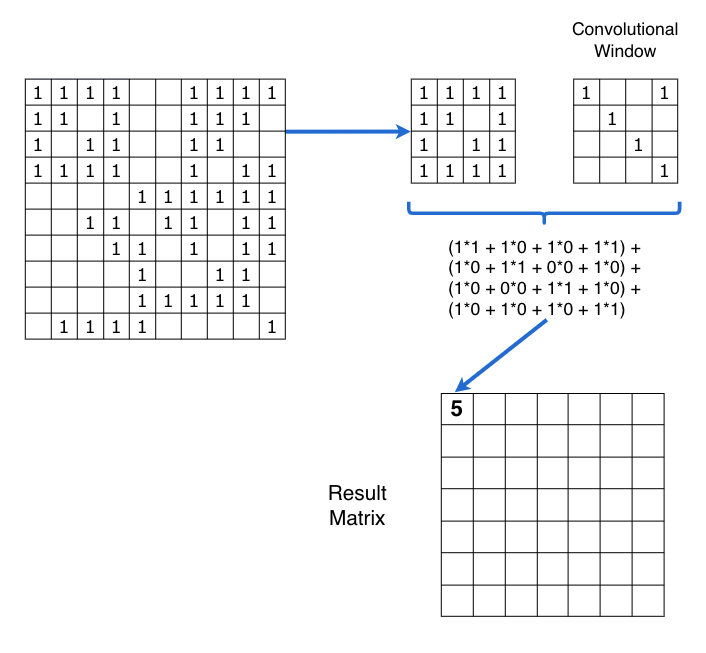
\includegraphics[width=0.9\columnwidth]{books/artificial-neural-network/chapter05/figure/convolution_example.png}
    		\centering
    	\caption{Hình ảnh minh họa quá trình nhân tích chập cho phần tử đầu tiên}
    	\label{fig:ConvolutionExample}
    \end{figure}

Xét một hình ảnh được biểu diễn dưới dạng ma trận \textit{I }kích thước 10x10 gồm các chữ số 1 (các vị trí không có số 1 được hiểu là 0) và một cửa sổ tích chập \textit{K} (cửa sổ trượt) là ma trận 4x4 như hình \ref{fig:ConvolutionSample}. Ta có công thức tính một phần tử của ma trận kết quả từ phép tích chập như sau:

\begin{equation}
S_{ij} = (I * K)_{ij} =  \sum_{m} \sum_{n} I(m,n)K(i-m,j-n)
\end{equation}

với \textit{i, j} là vị trí dòng và cột của phần tử kết quả,\textit{ m} và \textit{n} là kích thước của ma trận hình ảnh [\ref{refer:17}].

Để dễ hình dung hơn về phép tích chập, ta sẽ xét ví dụ trên bằng cách trực quan hóa thông qua hình ảnh. Ta thực hiện phép tích chập bằng cách trượt cửa sổ như sau:
\begin{itemize}
\item Nhân tích chập cửa sổ trượt với ma trận con 4x4 tại vị trí đầu tiên của ma trận hình ảnh. Phép nhân tích chập được thực hiện bằng cách nhân từng phân tử của ma trận hình ảnh con với phần tử tại ví trí tương ứng của cửa sổ trượt sau đó cộng các kết quả lại. Kết quả cuối cùng chính là giá trị của phần tử đầu tiên trong ma trận kết quả. Hình \ref{fig:ConvolutionExample} mô tả cụ thể quá trình này.
\item Trượt cửa sổ tích chập sang phải của ma trận hình ảnh một đơn vị cột và tiếp tục nhân tích chập để tìm được phần tử thứ 2 trong ma trận kết quả. Tiếp tục trượt sang phải cho đến khi không thể trượt thêm. Như vậy ta có được các phần tử của hàng đầu tiên cho ma trận kết quả tích chập.

\begin{figure}[!h]
    	\centering
    		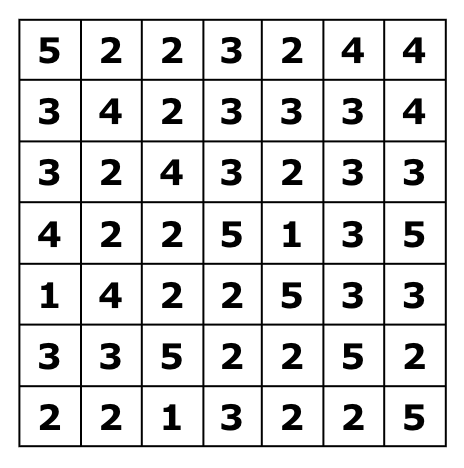
\includegraphics[width=0.4\columnwidth]{books/artificial-neural-network/chapter05/figure/convolution_filter_result_1.png}
    		\centering
    	\caption{Hình ảnh mô tả ma trận kết quả đầy đủ sau khi nhân tích chập với cửa sổ trượt đầu tiên}
    	\label{fig:ConvolutionExampleResult}
    \end{figure}

\item Để tính tiếp hàng thứ 2 cho ma trận kết quả, ta dời cửa sổ trượt về vị trí ban đầu và trượt cửa sổ xuống một đơn vị hàng. Tiếp tục lặp lại quá trình nhân tích chập và trượt cửa sổ. Ma trận kết quả sau khi hoàn thành quá trình tích chập sẽ có kích thước 7x7 như hình \ref{fig:ConvolutionExampleResult}.
\end{itemize}

\begin{figure}[!h]
	\centering
		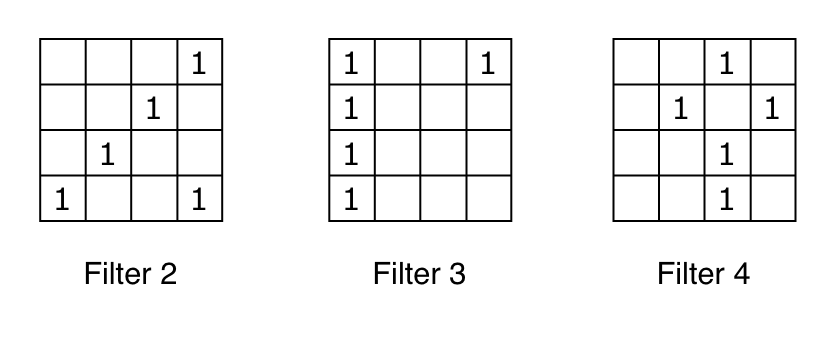
\includegraphics[width=0.8\columnwidth]{books/artificial-neural-network/chapter05/figure/convolution_filter_2_3_4.png}
		\centering
	\caption{Hình ảnh mô tả 3 cửa sổ trượt tiếp theo}
	\label{fig:ConvolutionSample234}
\end{figure}

\begin{figure}[!h]
	\centering
		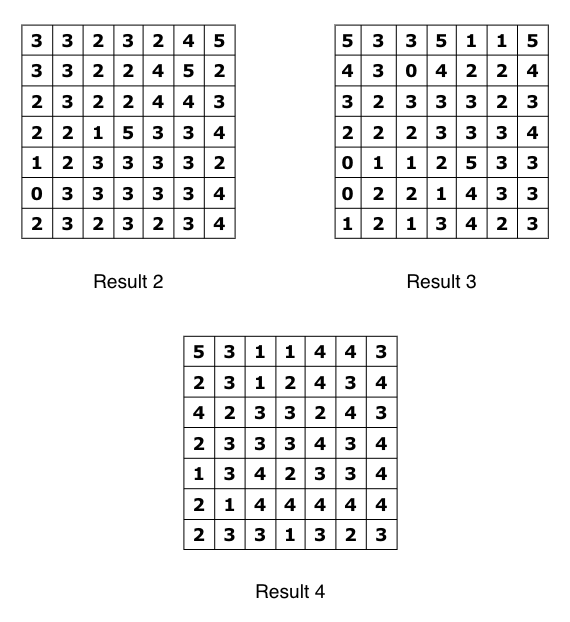
\includegraphics[width=0.8\columnwidth]{books/artificial-neural-network/chapter05/figure/convolution_filter_result_2_3_4.png}
		\centering
	\caption{Hình ảnh mô tả 3 ma trận kết quả sau khi nhân tích chập từ 3 cửa sổ trượt trên}
	\label{fig:ConvolutionResult234}
\end{figure}

Như vậy, ta đã có thể nắm được quá trình nhân tích chập diễn ra như thế nào.

Để thực hành làm quen với phép tích chập, ta hãy tiếp tục nhân tích chập ma trận hình ảnh ban đầu cho các cửa sổ trượt 2,3 và 4 như trong hình \ref{fig:ConvolutionSample234}. Kết quả nhận được sẽ giống với 3 ma trận kết quả trong hình \ref{fig:ConvolutionResult234}.


\subsection{Phép gộp (Pooling)}
\hspace{\parindent} Sau khi có được các ma trận kết quả với kích thước 7x7 từ phép tính tích chập. Ta tiếp tục thực hiện \textit{phép gộp} (pooling) để tiếp tục thu nhỏ ma trận hình ảnh. Có nhiều cách thực hiện phép gộp khác nhau như: lấy giá trị lớn nhất (max pooling), lấy giá trị trung bình (averrage pooling) hay lấy giá trị tổng (sum pooling). Trong thực tế, max pooling có khả năng khử nhiễu tốt hơn các loại pooling khác, vì vậy ta sẽ sử dụng max pooling để làm ví dụ minh họa cho phép gộp.

\begin{figure}[!h]
	\centering
		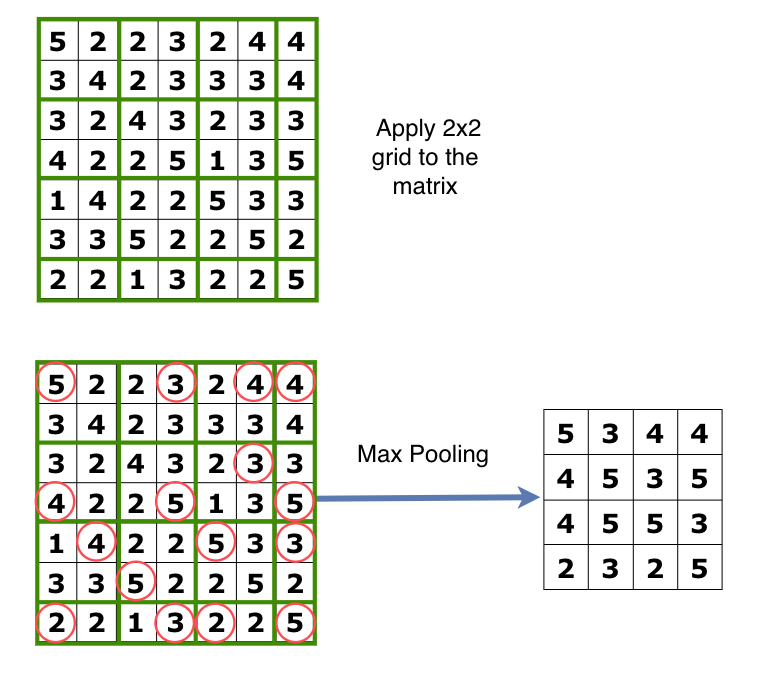
\includegraphics[width=0.8\columnwidth]{books/artificial-neural-network/chapter05/figure/max_pooling_example.png}
		\centering
	\caption{Hình ảnh minh họa quá trình thực hiện phép gộp max pooling}
	\label{fig:MaxPoolingExample}
\end{figure}

Xét ma trận kết quả được tính từ cửa sổ tích gộp đầu tiên. Ta thực hiện phép gộp max pooling như sau (hình \ref{fig:MaxPoolingExample} mô tả quá trình thực hiện phép gộp này):
\begin{itemize}
\item Chia ma trận kết quả ra thành các ma trận con (grid) có kích thước 2x2. Lưu ý là do ma trận kết quả có kích thước là 7x7 nên các ma trận con nằm ở cuối hàng và cuối cột chỉ có kích thước 1x2 hoặc 2x1.
\item Giá trị lớn nhất trong mỗi ma trận con (khoanh tròn màu đỏ) chính là phần tử của ma trận gộp mới. Lúc này ma trận kết quả sau khi gộp chỉ còn có kích thước 4x4, giảm đáng kể so với ma trận 10x10 ban đầu.
\end{itemize}

\begin{figure}[!h]
	\centering
		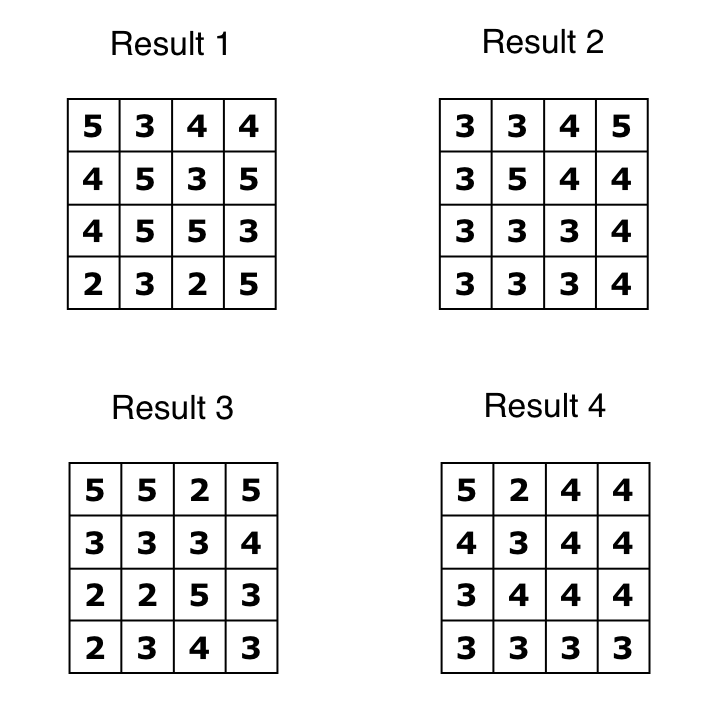
\includegraphics[width=0.6\columnwidth]{books/artificial-neural-network/chapter05/figure/max_pooling_results.png}
		\centering
	\caption{Hình ảnh mô tả 4 ma trận kết quả sau khi thực hiện max pooling}
	\label{fig:MaxPoolingResults}
\end{figure}

Tiếp tục thực hiện phép gộp dùng giá trị lớn nhất cho 3 ma trận kết quả tích chập còn lại, ta nhận được 4 ma trận kết quả tương ứng với 4 cửa sổ trượt ban đầu như hình \ref{fig:MaxPoolingResults}.

Như vậy, ta đã nắm bắt được ý tưởng của phép toán thứ 2 trong mạng nơ-ron tích chập đó là phép gộp (\textit{pooling}).

\subsection{Ý nghĩa của ma trận kết quả}
\hspace{\parindent} Sau khi đã thực hiện \textit{phép tích chập} (convolution) và \textit{phép gộp} (pooling), ta có được 4 ma trận kết quả kích thước 4x4 tương ứng với 4 cửa sổ trượt (hình \ref{fig:MaxPoolingResults}). Ta nhận thấy giá trị tối đa có thể có được của mỗi phần tử là 5. Do đó, ta thực hiện thêm một biến đổi cho 4 ma trận này bằng cách chuyển các giá trị 5 thành dấu x, các giá trị nhỏ hơn 5 đều được thay bằng 0. Sau phép biến đổi này, ta có được 4 ma trận mới như hình \ref{fig:CNNResultsMeaning}.

\begin{figure}[!h]
	\centering
		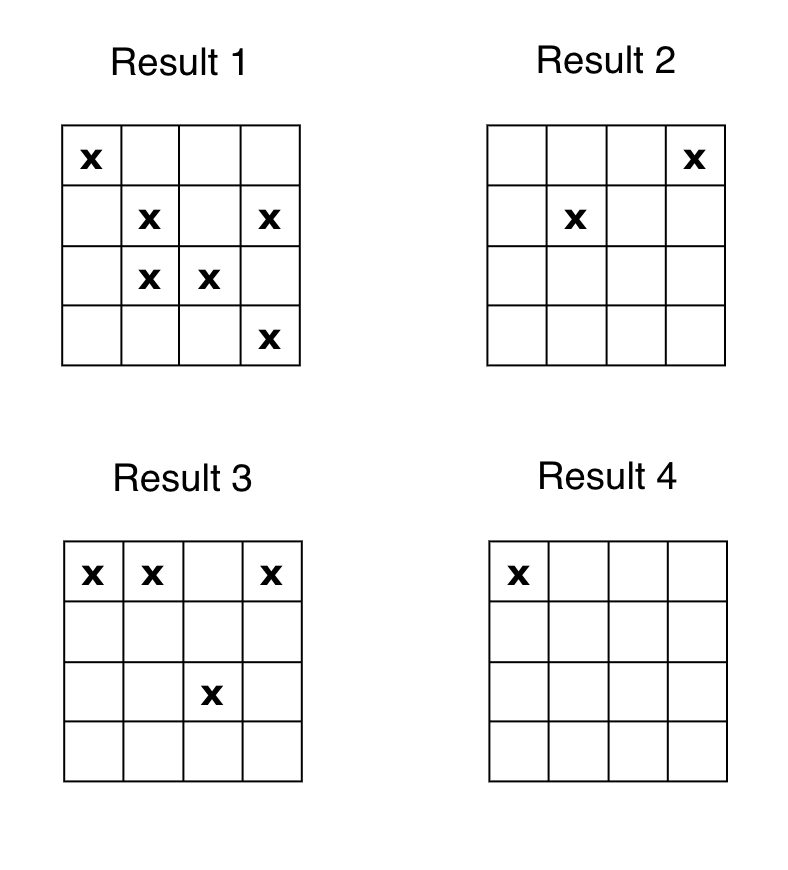
\includegraphics[width=0.6\columnwidth]{books/artificial-neural-network/chapter05/figure/cnn_results_meaning.png}
		\centering
	\caption{Hình ảnh mô tả 4 ma trận kết quả mới sau khi lượt giảm các giá trị nhỏ hơn 5}
	\label{fig:CNNResultsMeaning}
\end{figure}

Có thể thấy, sau khi biến đổi thì các ma trận kết quả đang thể hiện được sự phân bố mẫu (pattern) của các cửa sổ trượt nhỏ trên ma trận hình ảnh ban đầu. Ví dụ như cửa sổ đầu tiên thể hiện một đường chéo các số 1 (xem lại hình \ref{fig:ConvolutionExample}) thì ma trận kết quả thể hiện phân bố đúng như bản chất ma trận hình ảnh gốc, với một đường chéo chạy dài từ đầu đến cuối. Hay như ma trận thứ 4, cửa sổ trượt thể hiện một hình tương tự mũi tên bị khuyết ở giữa và nằm lệch về bên phải (xem hình \ref{fig:ConvolutionSample234}). Ở ma trận gốc thì hình này chỉ xuất hiện đúng một lần tại góc trên cùng bên trái của hình ảnh.

Từ quan sát này, ta có thể hiểu được vì sao các cửa sổ trượt này được gọi là các \textit{bộ lọc} (filter). Nhiệm vụ của chúng chính là tìm ra các đặc trưng của hình ảnh. Ở các lớp cao hơn, các bộ lọc đóng các vai trò khác nhau tùy theo yêu cầu của bài tóan như bộ phát hiện cạnh (edge detector), bộ phát hiện nhiễu (noise detector),...

\subsection{Bản đồ thuộc tính (Feature map)}
\begin{figure}[!h]
	\centering
		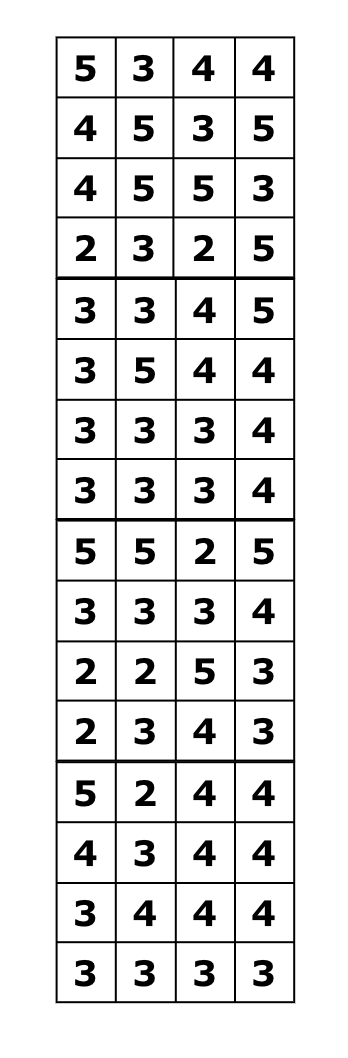
\includegraphics[width=0.3\columnwidth]{books/artificial-neural-network/chapter05/figure/feature_map.png}
		\centering
	\caption{Hình ảnh mô tả bản đồ thuộc tính từ việc ghép các ma trận kết quả}
	\label{fig:feature_map}
\end{figure}

\hspace{\parindent} Nếu ghép 4 ma trận kết quả ở hình \ref{fig:MaxPoolingResults} lại với nhau, ta được một hình ảnh như hình \ref{fig:feature_map}. Đây được gọi là \textit{bản đồ thuộc tính} (feature map), được trích xuất sau quá trình tích chập của mạng CNN. Bản đồ thuộc tính là một đặc trưng nổi bật của mạng nơ-ron tích chập, bởi nó thể hiện được các \textit{thuộc tính tiềm ẩn }(latent features) của hình ảnh đầu vào.

Cần lưu ý rằng \textit{bản đồ thuộc tính} được sinh ra dựa trên các \textit{bộ lọc} đã được định nghĩa trước (hay chính là các cửa sổ tích chập trong ví dụ trên). Do đó, điều quan trọng chính là làm sao định nghĩa được các \textit{bộ lọc} này một cách phù hợp để áp dụng hiệu quả cho những bài toán cụ thể. Ví dụ như với bài toán nhận diện khuôn mặt người, \textit{bộ lọc} sẽ là các bộ nhận diện mắt, mũi, miệng. Còn đối với bài toán nhận diện vạch kẻ đường, mạng nơ-ron cần học được các \textit{bộ lọc} nhận diện đường thẳng,... Vấn đề này sẽ được bàn đến trong phần tiếp theo, khi ta cần sử dụng cơ chế học của \textit{mạng nơ-ron nhân tạo} thông thường để có thể học được \textit{bộ lọc}.

\section{Mạng nơ-ron tích chập dưới góc nhìn của một mạng nơ-ron nhân tạo}
\hspace{\parindent} Trong một mạng nơ-ron nhân tạo thông thường thì một mạng nơ-ron được cấu thành bởi các nút nơ-ron khác nhau nối tiếp nhau và qua quá trình xử lý thông tin sẽ tạo ra các nút nơ-ron ở tầng tiếp theo. Tương tự như vậy với mạng nơ-ron tích chập, ví dụ có một hình ảnh được biểu diễn dưới dạng ma trận đầu vào với kích thước 10x10 và một cửa sổ tích chập là ma trận 4x4 thì quá trình nhân tích chập tại vị trí đầu trên ma trân đầu vào 10x10 sẽ tạo ra được một phần tử của ma trận mới và đó cũng tương đương với một nút nơ ron được tạo ra sau khi thực hiện một phép biến đổi. Nút nơ-ron mới sẽ nối với 16 điểm trên ma trận đầu vào.

\begin{figure}[!h]
	\centering
		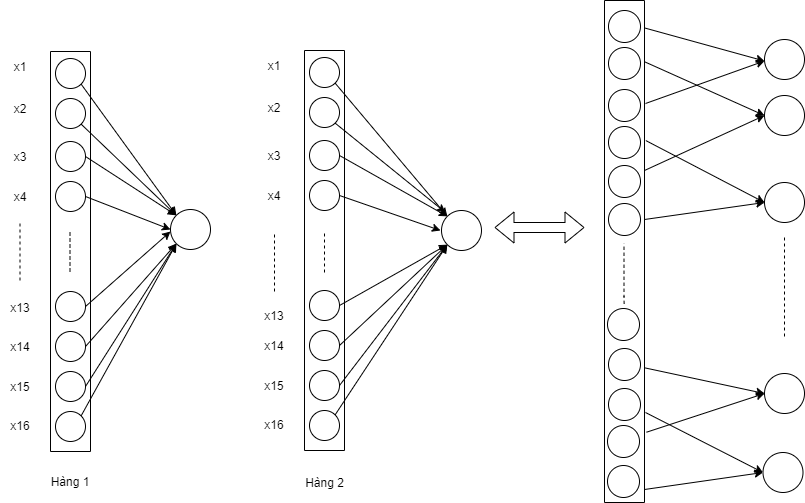
\includegraphics[width=0.8\columnwidth]{books/artificial-neural-network/chapter05/figure/cnn_filter.png}
		\centering
	\caption{Hình ảnh mô tả phân tích chập một bộ lọc tạo ra các nơ-ron}
	\label{fig:CNN}
\end{figure}

Hình \ref{fig:CNN} mô tả một ma trận đầu vào cùng với một cửa sổ và khi thực hiện phép tích chập trên một vị trí trên ma trận đầu vào sẽ tạo ra được một nút nơ-ron. Khi cho cửa sổ trượt qua hàng thứ hai sẽ thu được một nơ-ron khá và khi ta cho ma trận filter này trượt hết trên ma trận đầu vào thì sẽ tạo ra được 49 nút nơ ron khác nhau và mỗi nút nối với một ma trận 16 đơn vị.


Một đặc điểm quan trọng của mạng nơ-ron tích chập là \textit{cơ chế chia sẻ trọng số} (shared weights). Có nghĩa là các trọng số trên mỗi bộ lọc phải giống nhau và các nơ-ron trong lớp ẩn đầu sẽ phát hiện chính xác điểm tương tự chỉ ở các vị trí khác nhau trong dữ liệu đầu vào. Việc làm này sẽ làm giảm tối đa số lượng các \textit{tham số} (parameters), mỗi bản đồ đặc trưng sẽ giúp phát hiện thêm một vài đặc trưng khác.
Với một ma trận hình ảnh đầu vào kích thước 10x10 như ở trên và 4 bộ lọc có ma trận kích thước 4x4 thì mỗi bản đồ thuộc tính cần 4×4 = 16 trọng số và số nơ-ron được tạo ra ở lớp thứ hai là 49. Như vậy nếu có 4 bản đồ thuộc tính thì có 4x16 = 64 tham số. Với một mạng nơ-ron có kết nối đầy đủ thì chúng ta sẽ có 10x10x49 = 4900 trọng số. Từ kết quả cho thấy sử dụng lớp tích chập sẽ cần số lượng tham số ít hơn nhiều lần so với lớp kết nối đầy đủ nhưng vẫn có thể rút ra các đặc trưng một cách hiệu quả.

Một khả năng khác của mạng nơ-ron tích chập là số tham số không phụ thuộc vào kích thước của đầu vào. Với những ma trận đầu vào có kích thước khác nhau và thông qua quá trình học theo phương pháp nơ-ron tích chập sẽ rút ra những thuộc tính ẩn mà ta có thể khó nhận thấy. Xét một ví dụ chúng ta có 10 bộ lọc và mỗi một bộ lọc sẽ là một ma trận kích thước 3x3x3 và có một giá trị sai lệch là 1, chúng ta cần tính xem có bao nhiêu parameter sẽ được tạo ra từ việc sử dụng mạng nơ-ron tích chập? Để giải được bài toàn này thì cần tính số lượng parameters cần dùng mỗi bộ lọc rồi từ đó tính được kết quả.

\begin{itemize}
    \item Số lượng tham số cho mỗi bộ lọc là 3x3x3 = 27
    \item Tổng số tham số cho mỗi bộ lọc là 27 +1 = 28
    \item Tổng số tham số cho 10 bộ lọc là 28 x 10 = 280
\end{itemize}

Như vậy từ ví dụ này thì cho dù dữ liệu đầu vào là bao nhiêu thì số lượng tham số được tạo ra cũng là 280, do đó số tham số có được từ mạng nơ-ron tích chập này không phụ thuộc vào kích thước đầu vào.

\section{Bài tập}
\begin{exer}
\label{chp05:exer1}
Cho ma trận hình ảnh kích thước 10x10 và một cửa sổ tích chập kích thước 4x4 như hình \ref{fig:CNNExercise1}. Hãy cho biết ma trận kết quả cụ thể và số chiều của ma trận này sau khi thực hiện phép tích chập và phép gộp max pooling.

\begin{figure}[!h]
	\centering
		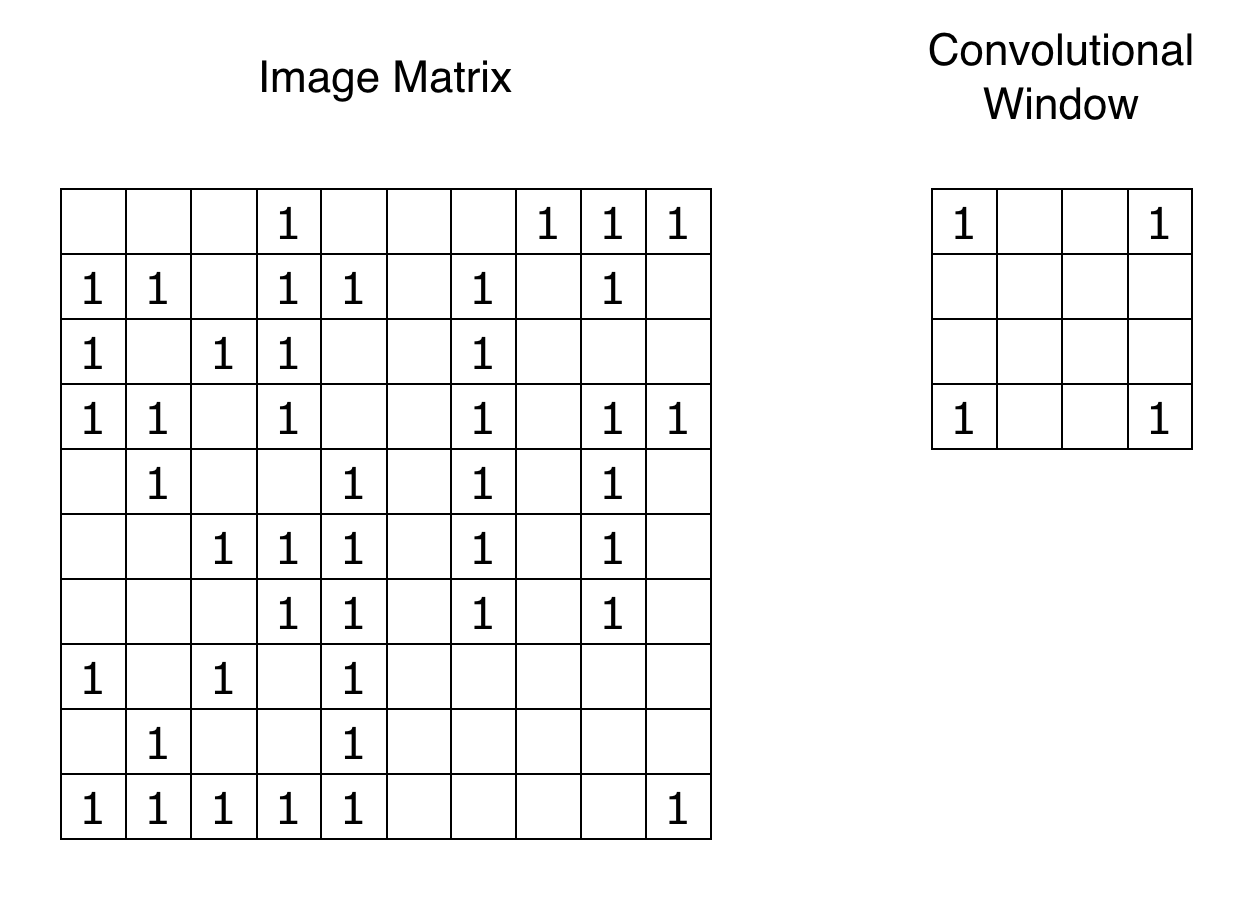
\includegraphics[width=0.8\columnwidth]{books/artificial-neural-network/chapter05/figure/cnn_exercise_1.png}
		\centering
	\caption{Ma trận hình ảnh và cửa sổ tích chập trong bài tập \ref{chp05:exer1}}
	\label{fig:CNNExercise1}
\end{figure}
\end{exer}

\begin{exer}
\label{chp05:exer2}
Cho một mạng nơ ron có 3 tầng, với tầng thứ nhất là một ma trận kích thước 10x10 và có 2 cửa sổ trượt ở tầng 1 như hình \ref{fig:CNNExercise2a} và ở tầng thứ hai có 1 cửa sổ trượt như hình \ref{fig:CNNExercise2b}. Hãy cho biết ở tầng thứ 3 sẽ là vector có bao nhiêu chiều?
% \clearpage
\begin{figure}[!h]
	\centering
		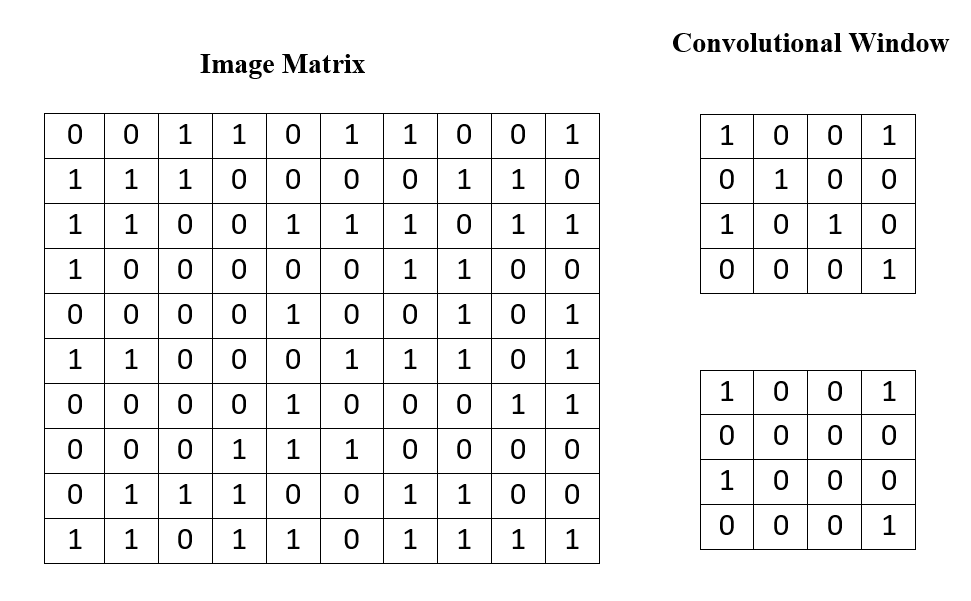
\includegraphics[width=1.0\columnwidth]{books/artificial-neural-network/chapter05/figure/exercise2a.png}
		\centering
	\caption{Ma trận hình ảnh và 2 cửa sổ tích chập ở tầng đầu tiên trong bài tập \ref{chp05:exer2}}
	\label{fig:CNNExercise2a}
\end{figure}
\begin{figure}[!h]
	\centering
		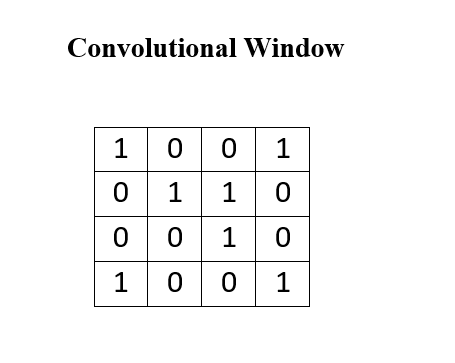
\includegraphics[width=0.6\columnwidth]{books/artificial-neural-network/chapter05/figure/exercise2b.png}
		\centering
	\caption{Cửa sổ tích chập cho tầng thứ 2 trong bài tập \ref{chp05:exer2}}
	\label{fig:CNNExercise2b}
\end{figure}
\end{exer}

\begin{exer}
Với cách làm cho bài tập \ref{chp05:exer2} thì ta vẫn cần ma trận ban đầu có số chiều cố định. Nếu chiều dài không cố định thì kết quả sẽ như thế nào?
\end{exer}

% \chapter{Học sâu trong xử lý ngôn ngữ tự nhiên}
\section{Triển khai một mạng CNN}
\hspace{\parindent} Một mạng CNN cơ bản bao gồm 3 bộ phận chính: \textit{Tầng tích chập} (Convolution),  \textit{tầng tổng hợp} (Pooling) và tầng cuối cùng là \textit{tầng kết nối đầy đủ} (Fully Connected).

Tầng tích chập là tầng quan trọng nhất và cũng là tầng đầu tiên của của mô hình CNN, có chức năng chính là phát hiện các đặc trưng cụ thể của input ban đầu (input ở đây có thể là một bức ảnh cây cối). Tầng này có các bộ phận chính là một ma trận đầu vào, \textit{bản đồ thuộc tính} (Feature map) và các \textit{cửa sổ trượt} (Convolution Filter). Tầng này bao gồm nhiều bản đồ thuộc tính đã được trích xuất ra các đặc tính cụ thể, mỗi bản đồ thuộc tính được tạo ra bằng cách quét input ban đầu qua cửa sổ trượt.

Tầng tổng hợp có mục đích làm giảm số lượng thông số mà ta phải tính toán, điều này giúp chúng ta giảm thời gian tính toán. Có 2 phương pháp tổng hợp thường gặp nhất là phép tổng hợp lớn nhất \textit{(Max pooling)} và phép tổng hợp trung bình \textit{(Average Pooling)}.

Cuối cùng tầng kết nối đầy đủ sẽ kết hợp các đặc điểm để ra được output của model.

Để dễ hình dung, ta sẽ mô tả mạng quá trình Convolution và Pooling ở ví dụ trước đó qua hình \ref{fig:convolutionexample7} dưới đây.

\begin{figure}[!h]
	\centering
		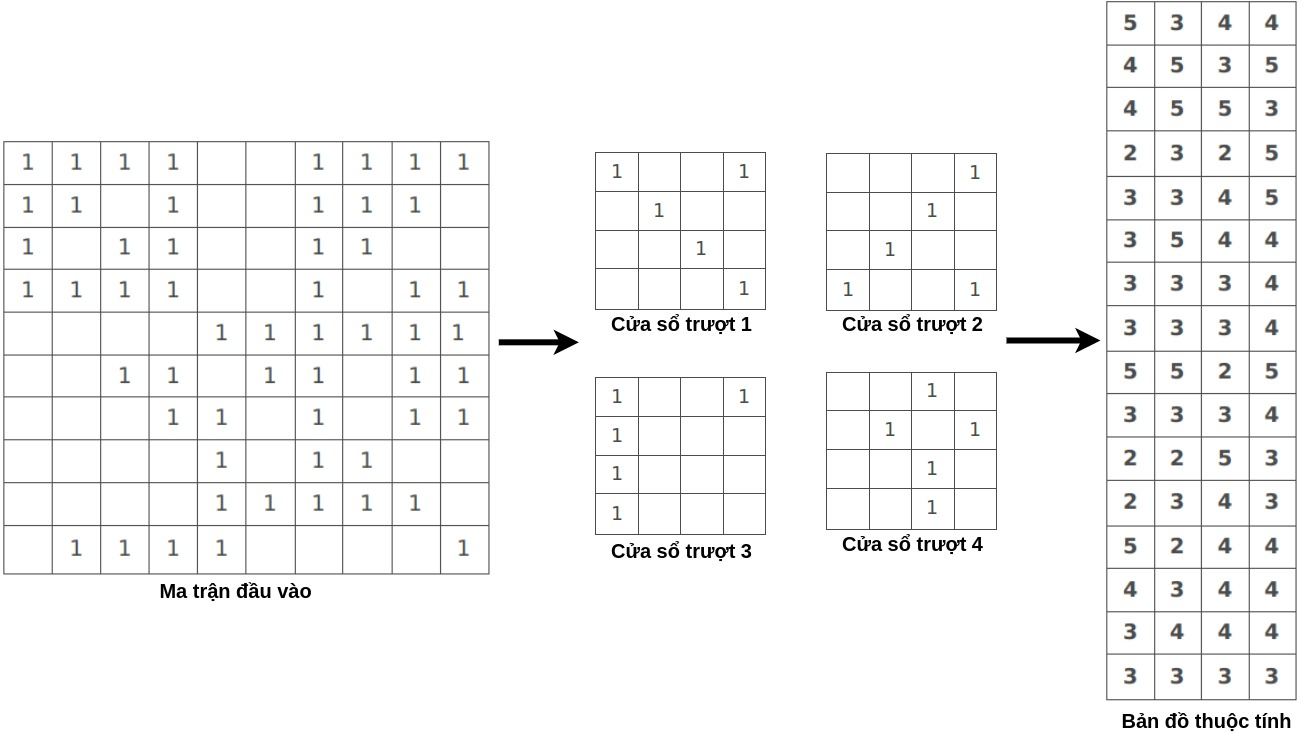
\includegraphics[width=1\columnwidth]{books/artificial-neural-network/chapter05/figure/convolution-example-7.jpg}
        \caption{Ví dụ một quá trình Convolution và Pooling}
        \label{fig:convolutionexample7}
\end{figure}

Hình \ref{fig:convolutionexample7} ở trên biểu diễn ví dụ một ma trận đầu vào có kích thước $10x10$, 4 cửa sổ trượt, mỗi cửa sổ trượt có kích thước $4x4$ và một bản đồ thuộc tính kết quả có kích thước $4x16$ và một bản đồ thuộc tính kết quả có kích thước $4x16$. Cách tính toán bao gồm nhân ma trận đầu vào với các cửa sổ trượt, sau đó thực hiện Pooling để ra được kết quả bản đồ thuộc tính đã được trình bày ở phần trước.

Đây là ví dụ quá trình một ma trận ban đầu được thực hiện Convolution và Pooling để thu được một bản đồ thuộc tính, và quá trình này có thể lặp đi lặp lại nhiều lần nếu cần thiết. Có nghĩa là, bản đồ thuộc tính $4x16$ ta có được trong ví dụ trên, có thể tiếp tục thực hiện qua các cửa sổ trượt khác, và sẽ thu được một bản đồ thuộc tính khác với cách tính toán tương tự. Quá trình này có thể lặp lại rất nhiều lần, và đến tầng cuối cùng thì ta sẽ học qua tầng Kết nối đầy đủ. Chúng ta cần chú ý rằng quá trình Convolution và Pooling phải được thực hiện ít nhất một lần và 2 tầng này luôn đi kèm với nhau, nhưng luôn cần một tầng kết nối đầy đủ sau cùng, điều này tương đương với việc triển khai một mạng Nơ-ron Network đơn giản cho một bài toán cần học.

Nhưng tại sao tầng cuối phải là Fully Connected? Ta có thể thấy thực ra việc học CNN là nó học các cái trọng số của các cửa sổ trượt, nó cần học và cập nhật lại các trọng số này. Tương tự như những bài toán trước đó, cần phải có bài toán cho nó học. Ví dụ, chúng ta có một lớp Fully Connected cho một bài toán rất đơn giản là nhập vào điểm toán, điểm văn,... sau đó dùng các dữ liệu điểm này để phân loại học sinh giỏi, học sinh khá,... thì bây giờ thay vì điểm toán, điểm văn,... output của chúng ta có rất nhiều thông số, và ta sẽ áp nó vào một lớp Fully Connected, kết quả output của nó sẽ thực hiện được rất nhiều mục đích khác nhau.

\begin{figure}[!h]
	\centering
		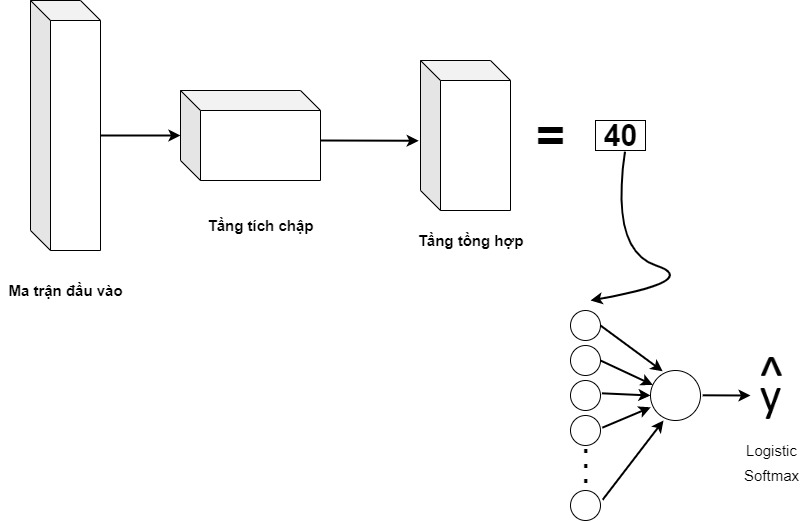
\includegraphics[width=1\columnwidth]{books/artificial-neural-network/chapter05/figure/convolution-example-5.jpg}
        \caption{Ví dụ một mạng CNN}
        \label{fig:convolutionexample5}
\end{figure}

Hình \ref{fig:convolutionexample5} thể hiện ví dụ một mạng CNN, ta có một ma trận đầu vào, một lớp tích chập và một lớp tổng hợp, ta ví dụ 40 là kết quả tính toán có được sau khi qua lớp tổng hợp, và giá trị 40 này sẽ được đưa vào lớp kết nối đầy đủ, sử dụng hàm logistic hoặc Softmax tùy theo mục đích, để thu được output sau cùng.

Và với kiến trúc mạng này, ta có thể ráp nhiều tầng CNN lại với nhau. Ta cũng chú ý rằng tầng kết nối đầy đủ có thể nhiều hơn 1 tầng để tăng khả năng học của bài toán cần triển khai, nhưng không nên quá nhiều vì sẽ làm mất đặc trưng của bài toán cần học, vì nếu quá nhiều sẽ dẫn đến việc tăng số lượng thông số đầu vào ,nếu quá nhiều thì chỉ riêng thông số của các tầng kết nối đầy dủ cũng đã hơn các tầng trước đó.

Mạng LeNet5 là một trong những mạng CNN lâu đời và nổi tiếng nhất, được Yann LeCUn phát triển vào những năm 1998. Cấu trúc của mạng LeNet5 gồm 2 lớp Convolution và Maxpooling, 2 lớp Fully Connected và output là hàm Softmax. Hình \ref{fig:lenetexample} thể hiện ví dụ một mạng Lenet5.

\begin{figure}[!h]
	\centering
		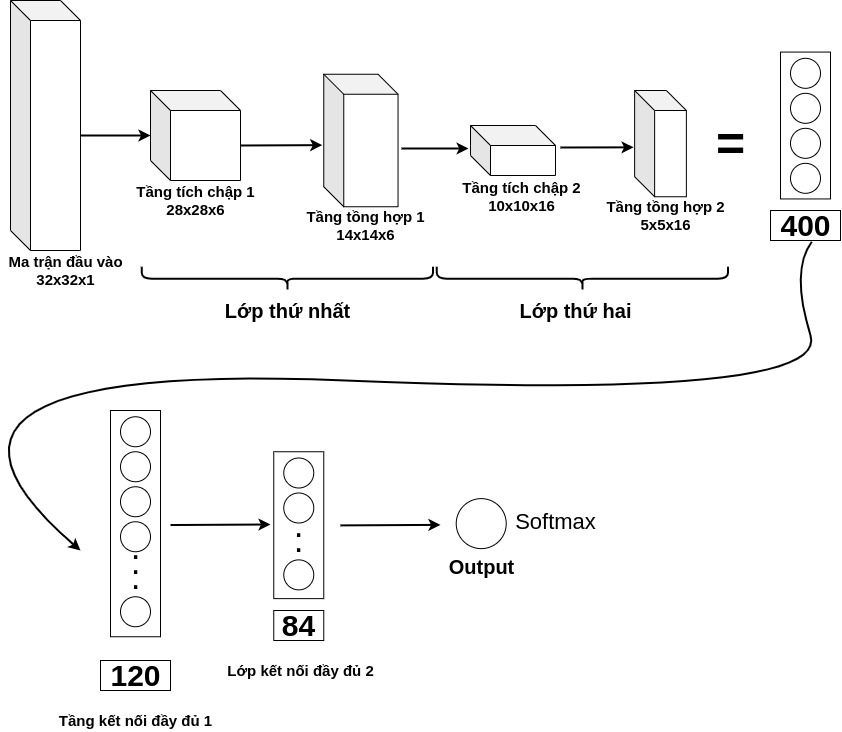
\includegraphics[width=1\columnwidth]{books/artificial-neural-network/chapter05/figure/lenet-example.jpg}
        \caption{Ví dụ một mạng Lenet-5}
        \label{fig:lenetexample}
\end{figure}

Một số thông tin về kiến trúc mạng Lenet5 như sau [\ref{refer:18}]:
\begin{itemize}
  \item Đầu vào là một ma trận có kích thước $32x32x1$, nghĩa là một tấm ảnh có chiều dài 32 pixel, chiều rộng ảnh là 32 pixel và số lượng kênh ảnh là 1 (ảnh đen trắng).
  \item Lớp thứ nhất bao gồm:
  \begin{itemize}
    \item Tầng tích chập thứ 1: là một ma trận $5x5x3$, tốc độ stride là 1, đi qua 6 cửa sổ trượt có kích thước $5x5x1$, và output của nó là 1 ma trận có kích thước $28x28x6$.
    \item Tầng tổng hợp thứ 1: Kích thước cửa sổ trượt là 1 ma trận $2x2$, tốc độ stride là 2, số lượng cửa sổ trượt là 16, và output của nó là 1 ma trận có kích thước $14x14x6$.
  \end{itemize}
  \item Lớp thứ hai bao gồm:
  \begin{itemize}
    \item Tầng tích chập thứ 2: là một ma trận $5x5x6$, tốc độ stride là 1, đi qua 16 cửa sổ trượt và output của nó là 1 ma trận có kích thước $10x10x16$.
    \item Tầng tổng hợp thứ 1: Kích thước cửa sổ trượt là 1 ma trận $2x2$, tốc độ stride là 2 và output của nó là 1 ma trận có kích thước $5x5x16$.
  \end{itemize}
  \item Giá trị Output của lớp thứ 2 sẽ là $5x5x16 = 400$.
  \item Giá trị Output của tầng kết nối đầy đủ thứ 1 sẽ là $120$.
  \item Giá trị Output của tầng kết nối đầy đủ thứ 2 sẽ là $84$.
\end{itemize}

Với kiến trúc như thế này, thì việc áp dụng vào từng bài toán cụ thể sẽ được trình bày ở phần sau.

\section{Sử dụng mạng CNN cho các bài toán NLP}
\label{sec6:introduction}
\subsection{Các cách tiếp cận cổ điển trước khi sử dụng CNN}
\textit{Xử lý ngôn ngữ tự nhiên} (Natural Language Processing - NLP) là một lĩnh vực nghiên cứu rất phong phú và sâu sắc, với rất nhiều kỹ thuật để trích xuất thông tin từ các ngôn ngữ. \textit{NLP} có rất nhiều ứng dụng phổ biến bao gồm \textit{phân loại tài liệu} (Text Classification), \textit{nhận dạng giọng nói} (Speech Recognition) và \textit{dịch vụ dịch thuật} (Translation Services). Với các bài toán này, ta hoàn toàn có thể sử dụng phương pháp cổ điển là Bag-of-Words và TF-IDF để giải quyết. Để ví dụ, ta phân tích 3 câu sau:
\begin{itemize}
  \item Câu 1: Bộ phim rất dở và dài.
  \item Câu 2: Bộ phim không dở và không dài.
  \item Câu 3: Bộ phim thật tệ và không vui.
\end{itemize}

\textbf{\textsc{Bag-of-words (BoW)}}

Đối với BoW, trước tiên chúng ta sẽ xây dựng một bộ từ điển bao gồm tất cả các từ khác nhau xuất hiện trong cả ba câu trên. Bộ từ điển này sẽ gồm 10 từ: [\textit{'Bộ', 'phim', 'rất', 'dở', 'và', 'dài', 'không', 'thật', 'tệ', 'vui'}].

Bây giờ chúng ta có thể lấy từng từ này và đánh dấu sự xuất hiện của chúng trong ba câu ở trên với 1 và 0. Điều này sẽ cung cấp cho chúng ta 3 vectơ cho 3 câu:

\begin{figure}[!h]
	\centering
		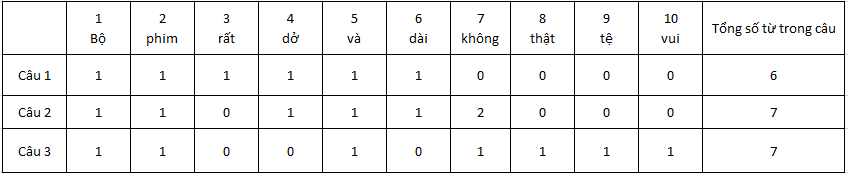
\includegraphics[width=1\columnwidth]{books/artificial-neural-network/chapter05/figure/BoW.PNG}
        \caption{Bảng biểu diễn sự xuất hiện của các từ trong câu}
        \label{fig:BoW}
\end{figure}

\begin{center}
    Vector biểu diễn cho câu 1:
    $\begin{bmatrix}
        1 & 1 & 1 & 1 & 1 & 1 & 0 & 0 & 0 & 0
    \end{bmatrix}$

    Vector biểu diễn cho câu 2:
    $\begin{bmatrix}
      1 & 1 & 0 & 1 & 1 & 1 & 2 & 0 & 0 & 0
    \end{bmatrix}$

    Vector biểu diễn cho câu 3:
    $\begin{bmatrix}
      1 & 1 & 0 & 0 & 1 & 0 & 1 & 1 & 1 & 1
    \end{bmatrix}$
\end{center}

Trong ví dụ trên, chúng ta có thể có các vector có độ dài 10. Tuy nhiên, chúng ta bắt đầu đối mặt với các vấn đề khi bắt gặp các câu mới:
\begin{enumerate}
  \item Nếu các câu mới chứa các từ mới, thì kích thước từ vựng của chúng ta sẽ tăng lên và do đó, độ dài của các vector cũng sẽ tăng theo.
  \item Ngoài ra, các vectơ cũng sẽ chứa nhiều 0, do đó dẫn đến một ma trận thưa (đó là những gì chúng tôi muốn tránh)
  \item Chúng ta chưa thể biểu diễn thông tin về ngữ pháp của các câu cũng như về thứ tự của các từ trong văn bản.
\end{enumerate}

\textbf{\textsc{TF-IDF}}

Chúng ta sẽ lại sử dụng cùng một bộ từ điển mà chúng ta đã xây dựng trong mô hình Bag-of-Words để chỉ ra cách tính toán đối với tần suất xuất hiện các từ của ba câu trên. Sau khi tính toán theo phương pháp TF-IDF, chúng ta được bảng như sau:

\begin{figure}[!h]
	\centering
		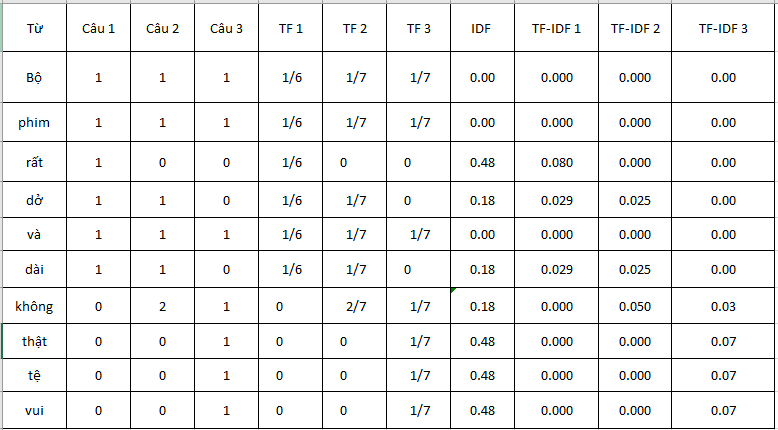
\includegraphics[width=1\columnwidth]{books/artificial-neural-network/chapter05/figure/tf-idf.PNG}
        \caption{Bảng biểu diễn cách tính TF-IDF đối với ba câu trên}
        \label{fig:sec6:tf-idf}
\end{figure}

Từ cách tính toán của TF-IDF trong hình \ref{fig:sec6:tf-idf} trên, ta nhận thấy các từ như \textit{'Bộ', 'phim', 'và' }  là những từ xuất hiện trong cả ba câu nhưng ít quan trọng, trong khi đó các từ còn lại quan trọng hơn nên có giá trị cao hơn. Vì vậy, những từ có giá trị cao hơn sẽ quan trọng hơn và những từ có giá trị thấp hơn thì ít quan trọng hơn. Bên cạnh đó, TF-IDF cũng cung cấp các giá trị lớn hơn cho các từ ít thường xuyên hơn và cao khi cả hai giá trị IDF và TF đều cao, nghĩa là từ này hiếm trong tất cả các tài liệu được kết hợp nhưng thường xuyên trong một tài liệu.

Từ ví dụ cho cả hai kỹ thuật Bag-of-words và TF-IDF, ta rút ra được kết luận như sau:
\begin{itemize}
  \item Bag of Words chỉ tạo ra một tập các vectơ chứa số lần xuất hiện từ trong tài liệu (đánh giá), trong khi mô hình TF-IDF chứa thông tin về các từ quan trọng hơn và cả những từ ít quan trọng hơn.
  \item Các vectơ Bag of Words rất dễ để giải thích. Tuy nhiên, TF-IDF thường hoạt động tốt hơn trong các mô hình học máy.
\end{itemize}

\subsection{Mô hình N-gram trong NLP}
Mặc dù cả Bag-of-Words và TF-IDF đều được sử dụng phổ biến theo cách riêng của của từng kỹ thuật, nhưng vẫn còn một vấn đề khá lớn, trong đó việc hiểu ngữ nghĩa và ngữ cảnh của các từ chính là vấn đề được quan tâm nhất. Cụ thể, vấn đề của Bag-of-words chính là nó chỉ quan tâm đến sự xuất hiện của từ đó trong câu mà không quan tâm đến thứ tự các từ trong câu đó. Còn TF-IDF, để phát hiện được sự giống nhau về ngữ nghĩa của hai từ đồng nghĩa, hoặc để dịch một câu sang ngôn ngữ khác, nó hầu như không làm được hoặc phải đòi hỏi cần nhiều thông tin hơn về các từ trong câu đó.

Từ những sự hạn chế đó, các kỹ thuật Word Embedding như Word2Vec, Continuous Bag of Words (CBOW), Skipgram,... sẽ thay thế chúng để biểu diễn thông tin N-gram. Mô hình N-gram là một trong những mô hình đơn giản nhất nhưng cũng quan trọng nhất để gán xác suất cho câu và cụm từ.

Trong lĩnh vực ngôn ngữ học hoặc tính toán xác suất, \textit{N-gram} là một chuỗi liên tục của $n$ mục được chứa trong một văn bản hoặc một câu nói. Các mục này có thể là âm vị, âm tiết, chữ cái hoặc từ. Trong NLP, N-gram được hiểu như một chuỗi gồm $N$ từ, theo cách hiểu đó, 2-gram là một chuỗi gồm 2 từ như "\textit{tôi đi}", "\textit{đi học}", và 3-gram là một chuỗi gồm 3 từ như "\textit{tôi đi học}".

Hãy bắt đầu với một xác suất có điều kiện $P(w|h)$, biểu diễn cho xác suất của một từ $w$ với điều kiện cho trước là một chuỗi từ $h$. Giả sử $h$ là câu "\textit{Hôm nay tôi đến thăm}", và chúng ta muốn tính xác suất của từ tiếp theo trong câu là từ "\textit{bác}", thì xác suất này sẽ được biểu diễn như sau:
\begin{center}
    $P(\textit{bác} | \textit{Hôm nay tôi đến thăm})$
\end{center}

Một cách để ước tính xác suất này là từ số lượng lặp lại tương đối: lấy một tập văn bản rất lớn, đếm số lần chúng ta thấy sự xuất hiện của câu "\textit{Hôm nay tôi đến thăm}", và đếm số lần mà từ tiếp theo của câu trên là "\textit{bác}". Phương pháp này sẽ trả lời cho câu hỏi có bao nhiêu lần từ "\textit{bác}" xuất hiện ngay phía sau câu "\textit{Hôm nay tôi đến thăm}":
\begin{center}
    $P(\textit{bác} | \textit{Hôm nay tôi đến thăm})$ =
    $\frac{C(\textit{Hôm nay tôi đến thăm bác})}{C(\textit{Hôm nay tôi đến thăm})}$
\end{center}

Tới đây, chúng ta có thể mường tượng ra rằng cách tính này hầu như là không khả thi khi thực hiện điều này trên toàn bộ kho văn bản, đặc biệt là kho văn bản có kích thước rất lớn. Để giải quyết vấn đề này, chúng ta sẽ sử dụng mô hình N-gram như một giải pháp khắc phục. Ở đây, thay vì tính xác suất trên toàn bộ kho văn bản, chúng ta sẽ ước chừng nó chỉ với một vài từ phía trước từ được dự đoán.

Trong mô hình bigram, để xấp xỉ xác suất xuất hiện của một từ đứng sau một chuỗi từ (được biểu diễn là $P(w_{n}|w^{n-1}_{1})$), nó sẽ chỉ sử dụng xác suất có điều kiện của một từ phía trước đó (được biểu diễn là $P(w_{n}|w_{n-1})$). Nói cách khác, ta sẽ tính
\begin{center}
    $P(\textit{bác} | \textit{thăm})$
\end{center}

thay vì tính cho
\begin{center}
    $P(\textit{bác} | \textit{Hôm nay tôi đến thăm})$
\end{center}

Khi chúng ta sử dụng mô hình bigram để dự đoán xác suất có điều kiện của từ tiếp theo, chúng ta sẽ có xấp xỉ sau:
\begin{center}
     $P(w_{n}|w^{n-1}_{1})$ $\approx$  $P(w_{n}|w_{n-1})$
\end{center}

% \textbf{\textsc{Sử dụng CNN vào bài toán NLP với phương pháp Word Embedding}}\\
\subsection{Sử dụng CNN vào bài toán NLP với phương pháp Word Embedding}
Với phương pháp Word Embedding, mỗi từ có thể biểu diễn thành một vector, từ đó một văn bản có thể giải thích thành một ma trận như hình bên dưới:
\begin{figure}[!h]
	\centering
		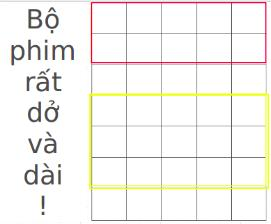
\includegraphics[width=0.3\columnwidth]{books/artificial-neural-network/chapter05/figure/convolution-example-8.jpg}
        \caption{Biểu diễn mỗi từ trong câu thành vector bằng Word Embedding}
        \label{fig:convolutionexample8}
\end{figure}

Từ hình \ref{fig:convolutionexample8} trên, ta để ý rằng hình chữ nhật màu đỏ sẽ biểu diễn một bi-gram trên ma trận này. Tương tự, hình chữ nhật màu vàng biểu diễn một tri-gram. Như vậy một bộ lọc ma trận (filter) $2xk$ là phù hợp để biểu diễn và rút trích các latent feature của các bi-gram, tương tự một bộ lọc ma trận $3xk$ cho tri-gram.

Với ma trận từ được biểu diễn như hình \ref{fig:convolutionexample8} ở trên, ta hoàn toàn có thể sử dụng như là input cho một mạng Nơron như bình thường, tuy nhiên với cách tiếp cận mới bằng các kỹ thuật Word Embedding, ta có thể sử dụng thêm tầng CNN để rút trích các latent features, được thể hiện như hình \ref{fig:convolutionexample9} ở dưới, và cách biểu diễn kinh điển của một tầng CNN sẽ được trình bày trong Case study tiếp theo.
\clearpage
\begin{figure}[!h]
	\centering
		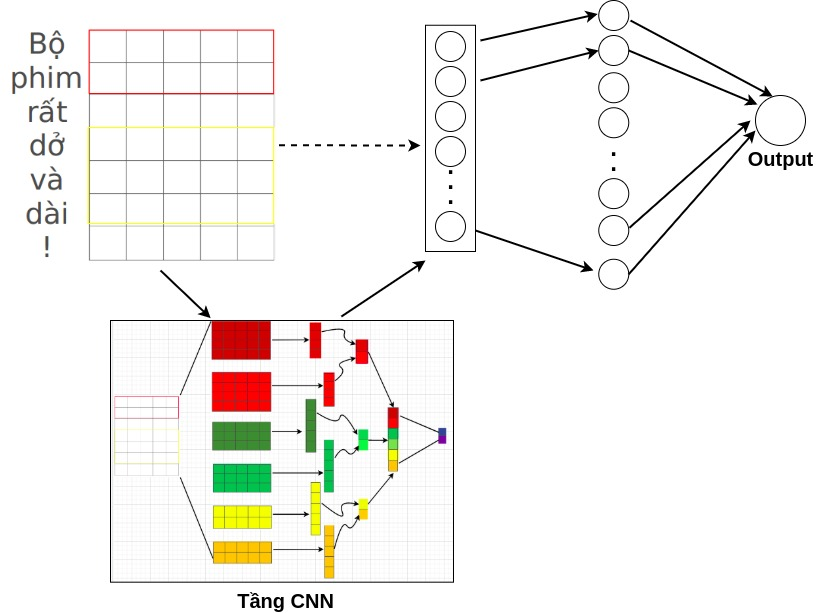
\includegraphics[width=1\columnwidth]{books/artificial-neural-network/chapter05/figure/convolution-example-9.jpg}
        \caption{Sử dụng thêm tầng CNN trong cách tiếp cận mới}
        \label{fig:convolutionexample9}
\end{figure}

\subsection{Case study: sử dụng CNN cho bài toán phân tích cảm xúc (sentiment analysis)}
Phân tích cảm xúc là quá trình phân tích, đánh giá quan điểm, cảm xúc của một người về một đối tượng nào đó qua lời nói hoặc văn bản (quan điểm có thể mang tính tiêu cực, tích cực hay bình thường,..). Sử dụng các kỹ thuật từ NLP, \textit{sentiment analysis} sẽ xem xét biểu thức của người dùng và lần lượt liên kết cảm xúc với những gì người dùng đã cung cấp. Tuy nhiên, cũng có trường hợp tùy thuộc vào nhiều yếu tố tác động mà một câu nói sẽ mang nhiều ý nghĩa cảm xúc khác nhau. \textit{sentiment analysis} được áp dụng rộng rãi cho việc phân tích đánh giá và phản hồi khảo sát, phương tiện truyền thông xã hội và trực tuyến và được sử dụng nhiều trong lĩnh vực dịch vụ chăm sóc khách hàng.

Trong phần này, chúng ta sẽ đi vào chi tiết một case study là
sử dụng CNN cho bài toán \textit{sentiment analysis}. Dưới đây là một sơ đồ biểu diễn kiến trúc CNN cho bài toán phân loại cảm xúc:

\begin{figure}[!h]
	\centering
		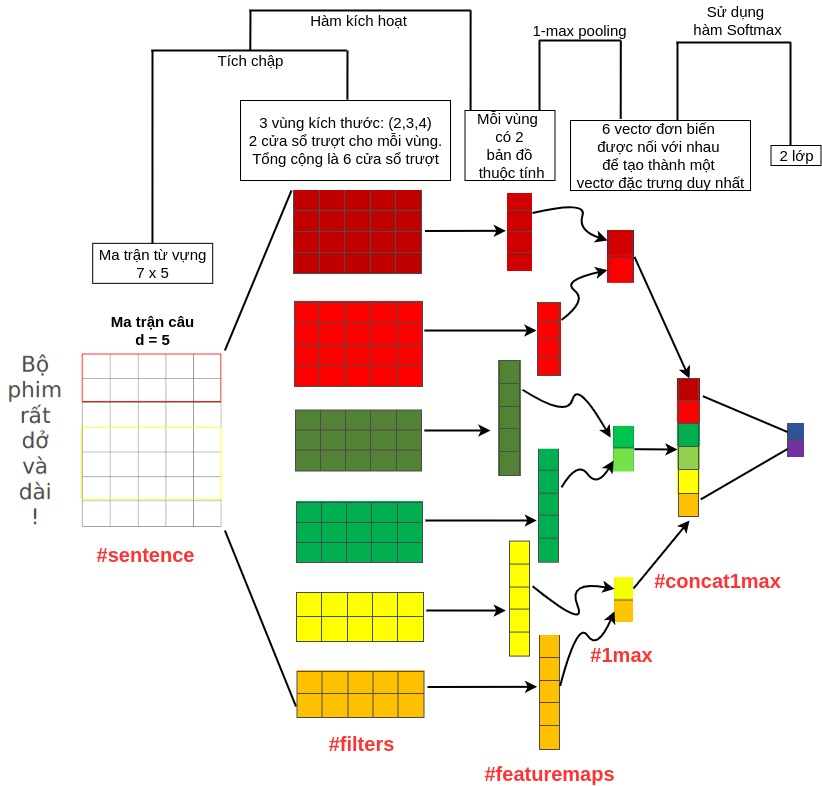
\includegraphics[width=1\columnwidth]{books/artificial-neural-network/chapter05/figure/convolution-example-10.jpg}
        \caption{Sơ đồ biểu diễn kiến trúc CNN cho bài toán phân loại cảm xúc}
        \label{fig:convolutionexample10}
\end{figure}

Để dễ hiểu, chúng ta sẽ chia sơ đồ trên ra thành 5 phần: \#sentence, \#filters, \#featuremaps, \#1-max và \#concat-1-max.

\textbf{\textit{\#sentence}}

Ví dụ là câu \textit{'Bộ phim rất dở và dài !'} tổng cộng có 7 từ trong câu (dấu chấm than vẫn được tính là một từ). Ở đây chúng ta chọn 5 là chiều của các vector từ. Chúng ta hãy biểu thị độ dài của câu là $s$ và $d$ là kích thước của vector từ, do đó chúng ta có một ma trận câu có hình dạng sxd là 7x5.

\textbf{\textit{\#filters}}

Một trong những đặc tính mong muốn của CNN là nó bảo toàn hướng không gian 2D trong thị giác máy tính. Thay vì 2 chiều, các văn bản có cấu trúc một chiều để biểu thị trình tự các từ. Vì chúng ta đã biểu diễn các từ trong câu ví dụ bằng các vector từ 5 chiều, do đó chúng ta sẽ sửa một chiều của bộ lọc để khớp với vector từ và thay đổi kích thước vùng $h$ \textit{(region size)}. \textit{Region size} đề cập đến số hàng của từ trong ma trận câu sẽ được lọc. Cụ thê ở đây,chúng ta sẽ chọn kích thước cho các bộ lọc được biểu diễn bởi các ma trận có số cột là 7, số hàng sẽ tùy biến (2, 3, 4) và chúng ta sẽ áp dụng 2 bộ lọc cho từng vùng, sau colvolution đầu tiên ta sẽ có 6 bộ lọc.

\textbf{\textit{\#featuremaps}}

Đối với phần này, chúng ta sẽ sử dụng CNN để thực hiện các phép toán tích chập, các công thức tính toán này đã được trình bày ở các phần trước đó.

\textbf{\textit{\#1-max}}

Ta đã biết được rằng chiều của $c$ phụ thuộc cả $s$ và $h$, nói cách khác, nó sẽ khác nhau giữa các câu có độ dài khác nhau và các bộ lọc có kích thước vùng khác nhau. Để giải quyết vấn đề này, chúng ta sẽ sử dụng hàm gộp 1-max và trích xuất số lớn nhất từ mỗi vector $c$.

\textbf{\textit{\#concat-1-max}}

Sau khi thực hiện phép gộp 1-max, chúng ta chắc chắn có một vector có độ dài cố định gồm 6 phần tử (= \textit{số bộ lọc} = \textit{số bộ lọc cho mỗi kích thước vùng (2)} x \textit{số lượng kích thước vùng được xem xét (3)}). Vector có chiều dài cố định này sau đó có thể được đưa vào một lớp softmax \textit{(fully-connected)} để thực hiện phân loại. Sự mất mát đến từ sự phân loại này sau đó sẽ được lan truyền ngược trở lại vào các tham số sau đây như là một phần của việc học:
\begin{itemize}
  \item Ma trận $w$ (ma trận dùng để tạo ra ma trận $o$).
  \item Bias được thêm vào $o$ để tạo ra ma trận $c$.
  \item Các vector từ.
\end{itemize}

Lớp softmax cuối cùng sau đó nhận vector tính năng này làm đầu vào và sử dụng nó để phân loại câu. Ở đây chúng ta giả định là phân loại nhị phân và do đó sẽ tạo ra hai trạng thái đầu ra có thể nhất.

Sau khi rút trích ra được các features, ta sẽ có vector output, và với vector này ta vẫn có thể sử dụng được cho các phương pháp học máy khác như SVM (Support Vector Machine), Naive Bayes,... Một cách tiếp cận rất kinh điển là ta sử dụng vector TF-IDF với SVM, hoặc với Nơron Network,... Nhưng tại sao đa phần rất thích sử dụng Nơron Network ở đây? Vì lúc đó chúng ta sẽ có một mạng end-to-end, đầu vào sẽ là một Nơron Network và đầu ra cũng là một Nơron Network. Sau khi có kết quả Loss ở tầng cuối cùng, nó có thể cập nhật toàn bộ các trọng số từ đầu bằng cơ chế Backpropagation. Toàn bộ các bước đều có thể học theo cơ chế Backpropagation, thay vì học từng khối thì ta có thể học từng cái Ngram, Trigram, Twogram,... Phần hiện thực mọi người có thể tham khảo một số mã nguồn mở như Github [\ref{refer:19}].

Trong thực tế, để lựa chọn kích thước và số lượng các bộ lọc cho các bài toán NLP áp dụng mạng CNN, chúng ta thường phải tham khảo từ các bài báo liên quan nổi tiếng trong ngành. Ở đây, chúng tôi giới thiệu một trong các bài báo tiêu biểu về việc lựa chọn các siêu tham số \textit{(hyperparameters)}như trong ví dụ trên, đó là bài báo \textit{'Convolutional Neural Networks for Sentence Classification'} của Yoon Kim (2014).

Trong bài báo, tác giả đã mô tả một loạt các thí nghiệm với các mạng CNN được xây dựng trong mô hình word2vec. Mặc dù có một ít sự điều chỉnh các \textit{hyperparameter}, nhưng đã thu được một mạng CNN đơn giản với một lớp chập thực hiện rất tốt. Kết quả của tác giả đã khẳng định cho một luận điểm rõ ràng rằng việc huấn luyện trước \textit{(pre-training)} các vector từ không được giám sát \textit{(unsupervised)} là một phần quan trọng trong việc ứng dụng học sâu cho NLP.

Cụ thể, qua tất cả các thực nghiệm về việc lựa chọn \textit{hyperparameter} trong bài báo, tác giả đã sử dụng: đơn vị tuyến tính đã chỉnh sửa \textit{(rectified linear units)}, cửa sổ bộ lọc ($h$) 3, 4, 5 đối với mỗi 100 feature map, tỉ lệ bỏ qua \textit{(dropout rate)} là $0.5$, ràng buộc $l_2$ cho các hàng của ma trận \textit{softmax} $s$ là 3 và mini-batch size = $50$. Các giá trị này được chọn thông qua tìm kiếm dạng lưới \textit{(grid search)} trên bộ dev SST-2 (Stanford Sentiment Treebank - đây là một phần mở rộng của thông số MR, Movie review với mỗi đánh giá tích cực/tiêu cực bằng một câu, nhưng có thêm các phân tách train/dev/test được cung cấp và các nhãn đánh giá \textit{(very positive, positive, neutral, negative, very negative)}).

Đối với thông số chiều cho các vector từ, ở đây tác giả tin rằng việc khởi tạo vector từ với những từ thu được từ mô hình ngôn ngữ noron không giám sát \textit{(unsupervised neural language model)} là một phương pháp phổ biến để cải thiện hiệu suất khi không có bộ đào tạo được giám sát lớn. Tác giả sử dụng các vector Word2Vec có sẵn công khai được đào tạo trên 100 tỷ từ trên Google News. Các vector này có chiều là 300 và được đào tạo bằng cách sử dụng kiến trúc CBOW \textit{(continuous bag-of-words)}. Các từ không có trong tập hợp \textit{pre-trained words} sẽ được khởi tạo ngẫu nhiên.

Trong bài báo này, tác giả cũng nhấn mạnh rằng trong suốt quá trình training, luôn tiếp tục kiểm tra hiệu suất trên bộ dev set và chọn trọng số chính xác cao nhất \textit{(highest accuracy weights)} cho lần đánh giá cuối cùng.

\section{Bài tập}
\begin{exer}
Cho câu sau đây:

Bộ phim rất dở và dài !

One-hot vector của câu này sẽ là
\begin{table}[!h]
    \centering
    \begin{tabular}{ |c|c|c|c|c|c|c|c|c| }
    \hline
         & Bộ & phim & rất & dở & và & dài & ! \\
    \hline
        Bộ & 1 & 0 & 0 & 0 & 0 & 0 & 0 \\
        phim & 0 & 1 & 0 & 0 & 0 & 0& 0 \\
        rất & 0 & 0 & 1 & 0 & 0 & 0 & 0 \\
        dở & 0 & 0 & 0 & 1 & 0 & 0 & 0 \\
        và & 0 & 0 & 0 & 0 & 1 & 0 & 0 \\
        dài & 0 & 0 & 0 & 0 & 0 & 1 & 0 \\
        ! & 0 & 0 & 0 & 0 & 0 & 0 & 1 \\
    \hline
    \end{tabular}
\end{table}

Ma trận Embedding của câu này sẽ là
$\begin{bmatrix}
    8 & 2 & 1 & 9 \\
    2 & 4 & 7 & 0 \\
    1 & 3 & 5 & 8 \\
    0 & 1 & 9 & 4 \\
    7 & 8 & 1 & 2
\end{bmatrix}$

Hãy cho biết ma trận biểu diễn câu này như thế nào ?
\end{exer}

\begin{exer}
Cho ma trận ban đầu là
$\begin{bmatrix}
    6 & 2 & 1 & 5 & 1 & 7 \\
    5 & 0 & 3 & 1 & 9 & 3 \\
    9 & 4 & 1 & 3 & 5 & 5 \\
    1 & 3 & 7 & 2 & 0 & 1 \\
\end{bmatrix}$

Ma trận 2-gram là
$\begin{bmatrix}
    1 & 5 & 9 & 3 \\
    3 & 8 & 0 & 2 \\
\end{bmatrix}$

Ma trận 3-gram là
$\begin{bmatrix}
    0 & 7 & 9 & 4 \\
    2 & 9 & 7 & 5 \\
    3 & 3 & 0 & 7
\end{bmatrix}$

Sử dụng Maxpooling, hãy cho biết bản đồ thuộc tính sau cùng được tạo ra.
\end{exer}

